%% ****** Start of file aiptemplate.tex ****** %
%%
%%   This file is part of the files in the distribution of AIP substyles for REVTeX4.
%%   Version 4.1 of 9 October 2009.
%%
%
% This is a template for producing documents for use with 
% the REVTEX 4.1 document class and the AIP substyles.
% 
% Copy this file to another name and then work on that file.
% That way, you always have this original template file to use.

%\documentclass[aip,graphicx]{revtex4-1}
%\documentclass[aip,reprint]{revtex4-1}

%\usepackage{graphicx}

%\draft % marks overfull lines with a black rule on the right
%\documentclass[pre,aps,floatfix,authordate1-4,twocolumn]{revtex4-1}
%\documentclass[pre,aps,floatfix,authordate1-4]{revtex4-1}

\documentclass[aps,prl,superscriptaddress,twocolumn]{revtex4}



%\documentclass[aps,prl,preprint,groupedaddress]{revtex4}

\usepackage{rotating} 
\usepackage{times}
\usepackage{graphicx}
\usepackage{setspace}
\usepackage{amsmath}
\usepackage{epstopdf}
\usepackage[obeyFinal]{easy-todo}
\begin{document}

% Use the \preprint command to place your local institutional report number 
% on the title page in preprint mode.
% Multiple \preprint commands are allowed.
%\preprint{}

\title{Quantitative quality of lipid-cholesterol interactions in atomistic resolution molecular dynamics simulations} %Title of paper

% repeat the \author .. \affiliation  etc. as needed
% \email, \thanks, \homepage, \altaffiliation all apply to the current author.
% Explanatory text should go in the []'s, 
% actual e-mail address or url should go in the {}'s for \email and \homepage.
% Please use the appropriate macro for the type of information

% \affiliation command applies to all authors since the last \affiliation command. 
% The \affiliation command should follow the other information.

\author{O. H. Samuli Ollila}
\email[]{samuli.ollila@aalto.fi}
%\homepage[]{Your web page}
%\thanks{}
%\altaffiliation{}
\affiliation{Aalto University}


% Collaboration name, if desired (requires use of superscriptaddress option in \documentclass). 
% \noaffiliation is required (may also be used with the \author command).
%\collaboration{}
%\noaffiliation

\date{\today}

\begin{abstract}
% insert abstract here
The quantitative quality of lipid-cholesterol interactions in atomistic resolution models will be determined against 
NMR and scattering data.
\end{abstract}

%\pacs{}% insert suggested PACS numbers in braces on next line

\maketitle %\maketitle must follow title, authors, abstract and \pacs

% Body of paper goes here. Use proper sectioning commands. 
% References should be done using the \cite, \ref, and \label commands


%\label{}
\section{Introduction}
The quantitative quality of lipid-cholesterol interactions in atomistic resolution models will be determined against 
NMR and scattering data.

\section{comparison of acyl chain order parameters between experiments and simulations}
Order parameters from simulations and experiments for acyl chains of 1-palmitoyl-2-oleoylphosphatidylcholine (POPC)
are shown in Fig. \ref{OrderParametersCHOL}.

\todo{Why are the order parameters of CHARMM36 too large compared to simulations even without cholesterol?}

\todo{Why there is decrease in order parameters towards beginning of acyl chain in MacRog model without cholesterol?}

\todo{Do the results suggests that condensation effect is too strong in MacRog model?}

 \begin{figure*}[]
  \centering
  \includegraphics[width=17.2cm]{../FIGS/OrderParametersCHOL.eps}

  \caption{\label{OrderParametersCHOL}
    Order parameters from simulations and experiments for acyl chains of  1-palmitoyl-2-oleoylphosphatidylcholine (POPC).}
  
\end{figure*}

\section{comparison of structure factors between experiments and simulations}

\todo{Structure factors should be calculated from the data with cholesterol
from CHARMM and MacRog simulations (the trajectories are in Zenodo). The calculations from Berger model should be checked
(data in https://github.com/NMRLipids/NmrLipidsCholXray/tree/master/scratch/POPCberger)}

\todo{The experimental data delivered by Georg Pabst and Peter Heftberger should be plotted
together with the simulation results. The data is already in https://github.com/NMRLipids/NmrLipidsCholXray/tree/master/DATA/POPC-Cholesterol}

\section{Conclusions}

% Tables may be be put in the text as floats.
% Here is an example of the general form of a table:
% Fill in the caption in the braces of the \caption{} command. Put the label
% that you will use with \ref{} command in the braces of the \label{} command.
% Insert the column specifiers (l, r, c, d, etc.) in the empty braces of the
% \begin{tabular}{} command.
%
% \begin{table}
% \caption{\label{} }
% \begin{tabular}{}
% \end{tabular}
% \end{table}

% If you have acknowledgments, this puts in the proper section head.
\begin{acknowledgments}
% Put your acknowledgments here.
\end{acknowledgments}

% Create the reference section using BibTe
\bibliography{refs.bib}

%\newpage
%\section{APPENDIX: The NMR results reported by Tiago Ferreira}

\listoftodos

\end{document}
%
% ****** End of file aiptemplate.tex ******
